\documentclass[landscape, 10pt, twocolumn]{article}
\usepackage[utf8]{inputenc}

\setlength{\parindent}{0in}

\usepackage[compact]{titlesec}
\titlespacing*{\section}{0pt}{0pt}{0pt}
\titlespacing*{\subsection}{0pt}{0pt}{0pt}

\usepackage{fancyhdr}
 
\pagestyle{fancy}

\usepackage[margin=0.5in,top=0.7in,footskip=.25in]{geometry}
\usepackage{float}
\usepackage{minted}
\usepackage{bm}
\setminted[python]{
    breaklines=true,
    mathescape=true,
    escapeinside=@@,
    encoding=utf8
}
\setminted[c]{
    breaklines=true,
    mathescape=true,
    escapeinside=||,
    encoding=utf8
}

% minted workaround
\makeatletter
\AtBeginEnvironment{minted}{\dontdofcolorbox}
\def\dontdofcolorbox{\renewcommand\fcolorbox[4][]{##4}}
\makeatother

\usepackage{tikz}
\usetikzlibrary{positioning}
\usetikzlibrary{arrows}
\usetikzlibrary{chains,fit,shapes}

 \everymath{\mathtt{\xdef\tmp{\fam\the\fam\relax}\aftergroup\tmp}}
 \everydisplay{\mathtt{\xdef\tmp{\fam\the\fam\relax}\aftergroup\tmp}}


\title{ŚCIAGA MRJPY}
\author{b.andysc }
\date{January 2019}

\newcommand{\ra}{\rightarrow}

\begin{document}


\section*{Changelog  $\ $} %  $\ $ is a hack so that math code is fixed-width font

\begin{itemize}
    \item \textbf{31.01.2020}
    
    \textbf{1.4 Liczenie Select}
    
    było: $\quad Select(X \ra bY) = \{ b, \#\}$
    
    powinno być: $\quad Select(X \ra bY) = \{ b \}$
    
    \item \textbf{03.02.2020}
    
    \textbf{1.6.2 LALR(1) / LR(1)}
    
    dodana uwaga o zmianie gramatyki
    
    reguła $S \ra aAa $ zamieniona na $S \ra Aa$
    
    \item \textbf{06.02.2021}
    
    \textbf{1.6.1 SLR(1)}
    
    przejście $1 \stackrel{S}{\ra} 2$ nie przesuwało kropki przy regule $S \ra \circ S u X$, a powinno
    
    dodatkowo spowodowało to dodanie dopełnienia $S$ do $2$, którego nie powinno być. To oznacza, że przejścia $2 \stackrel{a}{\ra} 9$ nie ma, za to powinno być przejście $1 \stackrel{a}{\ra} 9$
\end{itemize}

\newpage
$\\$
\newpage


\section{Parsery}

    $LR(0) \subseteq SLR(1) \subseteq LALR(1) \subseteq LR(1)$;  $\ \ \ \ \ $
$LL(1) \subseteq LR(1)$

\textsc{Na przykładzie:}

$\quad S \ra SuX\ |\ aX$

$\quad X \ra bY\ |\ b$

$\quad Y \ra aX$


\subsection{Przerabianie gramatyki na LL(1)}
\begin{itemize}
    \item Lewostronna rekurencja: $A \ra A \alpha\ |\ \beta$ zastępujemy przez $A \ra \beta A'$, $A' \ra \alpha A'\ |\ \varepsilon$
    
    $S \ra a X S'$
    
    $S' \ra uXS'\ |\ \varepsilon$
    \item "Wyciąganie przed nawias": $A \ra \alpha\ |\ \alpha B$ zastępujemy przez $A \ra \alpha C'$, $C' \ra \varepsilon$, $C' \ra B$
    
    $X \ra bY'$
    
    $Y' \ra \varepsilon$
    
    $Y' \ra aX$
\end{itemize}


\subsection{Liczenie First($\alpha$)}

$First(\alpha\beta\gamma) = \left\{ 
    \begin{array}{ll} 
        \alpha & gdy\ \alpha\ jest\ terminalem\ (w\ tym\ \varepsilon) \\
        First(\alpha) & gdy\ \alpha\ jest\ nieterminalem\\ & ORAZ\ \varepsilon\ nie\ nalezy\ do\ First(\alpha) \\
        First(\alpha)-\{\varepsilon \} \cup First(\beta\gamma) & gdy\ \alpha\ jest\ nieterminalem\\ & ORAZ\ \varepsilon\ nalezy\ do\ First(\alpha)
    \end{array}
\right.$

Do zbioru $First(A)$ dodajemy wszystkie Firsty prawych strony produkcji A. $\varepsilon \in First(ABC)$ wtedy gdy $\varepsilon$ należy do wszystkich firstów po prawej stronie.

\textsc{Przykład}:

$\quad First(S) = \{ a \}$

$\quad First(S') = \{ u, \varepsilon \}$

$\quad First(X) = \{ b \}$

$\quad First(Y') = \{ a, \varepsilon \}$

\subsection{Liczenie Follow($\alpha$)}

$A \ra \beta B\alpha$

$Follow(B) = First(\alpha)\ \cup\ \left\{ \begin{array}{ll}  Follow(A) & gdy\ \varepsilon \in First(\alpha)\ (takze\ gdy\ \alpha\ nie\ ma,\\ & tzn.\ jest\ \varepsilon) \\ \emptyset  & wpp  \end{array} \right.$

$\beta$ w ogóle nie ma znaczenia, może być $\varepsilon$, $\alpha$ też może być dowolna, składać się z terminali, nieterminali bądź być puste. W skrócie: żeby policzyć $Follow(B)$, patrzymy na wszystkie produkcje, gdzie $B$ jest po prawej stronie, lewa strona %nigdy nie zasypia%
nie ma znaczenia.

\textsc{Przykład}:

$\quad Follow(S) = \{ \# \}$ (do nieterminala startowego dajemy symbol końcowy)

$\quad Follow(S') = Follow(S) = \{ \# \}$

$\quad Follow(X) = Follow(Y') \cup First(S') \cup Follow(S) \cup Follow(S') = \{ u, \#\}$

$\quad Follow(Y') = Follow(X) = \{ u, \#\}$

\subsection{Liczenie Select($A \rightarrow \beta$)}

$Select(A \ra \alpha) = First(\alpha \cdot Follow(A))$ (jak $\alpha$ może być $\varepsilon$ to bierzemy Firsta oraz Follow, jak nie jest to bierzemy tylko First)

\textsc{Przykład}:

$\quad Select(Y' \ra \varepsilon) = \{ u, \#\}$

$\quad Select(S' \ra \varepsilon) = \{ \#\}$

$\quad Select(X \ra bY) = \{ b \}$

$\quad Select(S \ra aXS') = \{ a \}$

$\quad Select(Y' \ra aX) = \{ a \}$

$\quad Select(S' \ra uXS') = \{ u \}$

\subsection{Parsowanie zstępujące (top down) - LL(1)}
Gramatyka jest LL(1) wtw gdy dwie różne produkcje tego samego nieterminala mają nieprzecinające się zbiory.

\subsection{Parsowanie wstępujące (bottom up)}

\textbf{Redukcje w LR(0) - po wszystkich terminalach}
\begingroup
\begin{enumerate}
    \small
    \setlength{\itemsep}{1pt}
    \setlength{\parskip}{0pt}
    \setlength{\parsep}{0pt}
    \item Dodajemy produkcję początkową $Z \ra \circ S\#$
    \item Tworzymy stan z produkcją $Z$
    \item Tam gdzie jest $\circ$ przed nieterminalem, musimy dodać produkcję tego nieterminala (dopełnienie)
\end{enumerate}
\footnotesize{Uwaga: to jest tylko część grafu, ale nawet tutaj już widać, że nie jest LR(0), dlatego nie ma całości.}
\begin{figure}[H]

\tikzset{every picture/.style={line width=0.75pt}} %set default line width to 0.75pt        

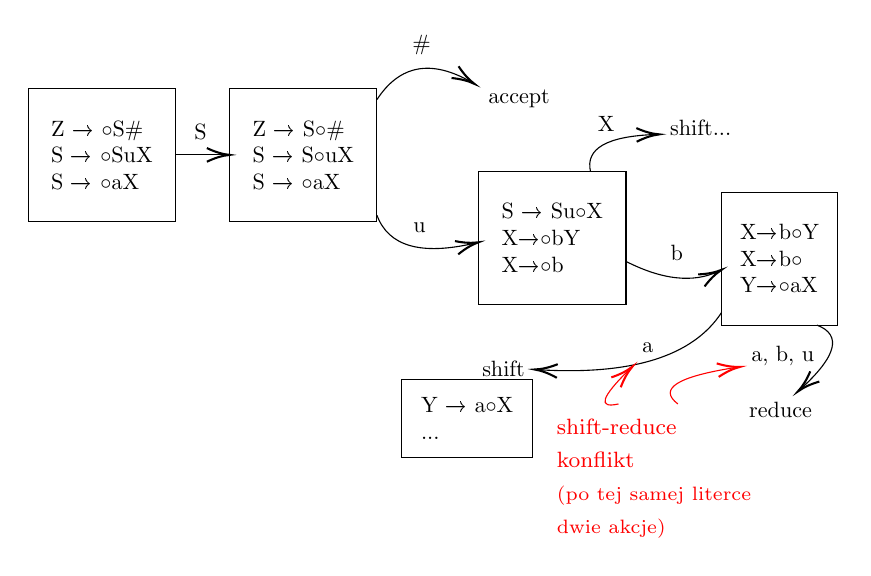
\begin{tikzpicture}[x=0.75pt,y=0.75pt,yscale=-1,xscale=1]

%uncomment if require: \path (0,300); %set diagram left start at 0, and has height of 300


% Text Node
\draw    (8,28) -- (79,28) -- (79,92) -- (8,92) -- cycle  ;
\draw (43.5,60) node [scale=0.8] [align=left] {Z → $\displaystyle \circ $S\#\\S → $\displaystyle \circ $SuX\\S → $\displaystyle \circ $aX};
% Text Node
\draw    (105,28) -- (176,28) -- (176,92) -- (105,92) -- cycle  ;
\draw (140.5,60) node [scale=0.8] [align=left] {Z → S$\displaystyle \circ $\#\\S → S$\displaystyle \circ $uX\\S → $\displaystyle \circ $aX};
% Text Node
\draw    (225,68) -- (296,68) -- (296,132) -- (225,132) -- cycle  ;
\draw (260.5,100) node [scale=0.8] [align=left] {S → Su$\displaystyle \circ $X\\X→$\displaystyle \circ $bY\\X→$\displaystyle \circ $b};
% Text Node
\draw    (342,78) -- (398,78) -- (398,142) -- (342,142) -- cycle  ;
\draw (370,110) node [scale=0.8] [align=left] {X→b$\displaystyle \circ $Y\\X→b$\displaystyle \circ $\\Y→$\displaystyle \circ $aX};
% Text Node
\draw (244.5,33) node [scale=0.8] [align=left] {accept};
% Text Node
\draw (237,163) node [scale=0.8] [align=left] {shift};
% Text Node
\draw (91,49) node [scale=0.8] [align=left] {S};
% Text Node
\draw (197.5,7) node [scale=0.8] [align=left] {\#};
% Text Node
\draw (320.5,107) node [scale=0.8] [align=left] {b};
% Text Node
\draw (306.5,153) node [scale=0.8] [align=left] {a};
% Text Node
\draw (370.5,183) node [scale=0.8] [align=left] {reduce};
% Text Node
\draw (371.5,157) node [scale=0.8] [align=left] {a, b, u};
% Text Node
\draw    (188,168) -- (251,168) -- (251,206) -- (188,206) -- cycle  ;
\draw (219.5,187) node [scale=0.8] [align=left] {Y → a$\displaystyle \circ $X\\...};
% Text Node
\draw (196.5,95) node [scale=0.8] [align=left] {u};
% Text Node
\draw (332,47) node [scale=0.8] [align=left] {shift...};
% Text Node
\draw (286.5,45) node [scale=0.8] [align=left] {X};
% Text Node
\draw (309.5,216) node  [align=left] {{\footnotesize \textcolor[rgb]{1,0,0}{shift-reduce}}\\{\footnotesize \textcolor[rgb]{1,0,0}{konflikt}}\\\textcolor[rgb]{1,0,0}{{\scriptsize (po tej samej literce}}\\\textcolor[rgb]{1,0,0}{{\scriptsize dwie akcje)}}};
% Connection
\draw    (79,60) -- (103,60) ;
\draw [shift={(105,60)}, rotate = 180] [color={rgb, 255:red, 0; green, 0; blue, 0 }  ][line width=0.75]    (10.93,-3.29) .. controls (6.95,-1.4) and (3.31,-0.3) .. (0,0) .. controls (3.31,0.3) and (6.95,1.4) .. (10.93,3.29)   ;

% Connection
\draw    (176,89.04) .. controls (181.56,104.13) and (197.36,108.61) .. (223.39,102.47) ;
\draw [shift={(225,102.08)}, rotate = 526.04] [color={rgb, 255:red, 0; green, 0; blue, 0 }  ][line width=0.75]    (10.93,-3.29) .. controls (6.95,-1.4) and (3.31,-0.3) .. (0,0) .. controls (3.31,0.3) and (6.95,1.4) .. (10.93,3.29)   ;

% Connection
\draw    (296,111.32) .. controls (313.43,120.16) and (328.19,121.8) .. (340.31,116.23) ;
\draw [shift={(342,115.39)}, rotate = 512.21] [color={rgb, 255:red, 0; green, 0; blue, 0 }  ][line width=0.75]    (10.93,-3.29) .. controls (6.95,-1.4) and (3.31,-0.3) .. (0,0) .. controls (3.31,0.3) and (6.95,1.4) .. (10.93,3.29)   ;

% Connection
\draw    (176,33.36) .. controls (186.96,16.6) and (202.13,13.79) .. (221.5,24.91) ;
\draw [shift={(223,25.79)}, rotate = 211.15] [color={rgb, 255:red, 0; green, 0; blue, 0 }  ][line width=0.75]    (10.93,-3.29) .. controls (6.95,-1.4) and (3.31,-0.3) .. (0,0) .. controls (3.31,0.3) and (6.95,1.4) .. (10.93,3.29)   ;

% Connection
\draw    (342,136.01) .. controls (328.14,157.13) and (298.6,166.28) .. (253.38,163.48) ;
\draw [shift={(252,163.39)}, rotate = 363.82] [color={rgb, 255:red, 0; green, 0; blue, 0 }  ][line width=0.75]    (10.93,-3.29) .. controls (6.95,-1.4) and (3.31,-0.3) .. (0,0) .. controls (3.31,0.3) and (6.95,1.4) .. (10.93,3.29)   ;

% Connection
\draw    (388,142) .. controls (400.19,146.69) and (397.57,156.94) .. (380.16,172.77) ;
\draw [shift={(378.79,174)}, rotate = 318.44] [color={rgb, 255:red, 0; green, 0; blue, 0 }  ][line width=0.75]    (10.93,-3.29) .. controls (6.95,-1.4) and (3.31,-0.3) .. (0,0) .. controls (3.31,0.3) and (6.95,1.4) .. (10.93,3.29)   ;

% Connection
\draw    (278.9,68) .. controls (276.37,56.95) and (286.79,51) .. (310.18,50.17) ;
\draw [shift={(312,50.11)}, rotate = 538.64] [color={rgb, 255:red, 0; green, 0; blue, 0 }  ][line width=0.75]    (10.93,-3.29) .. controls (6.95,-1.4) and (3.31,-0.3) .. (0,0) .. controls (3.31,0.3) and (6.95,1.4) .. (10.93,3.29)   ;

% Connection
\draw [color={rgb, 255:red, 255; green, 0; blue, 0 }  ,draw opacity=1 ]   (321,180) .. controls (311.33,172.63) and (320.74,166.76) .. (349.23,162.37) ;
\draw [shift={(351,162.11)}, rotate = 531.5899999999999] [color={rgb, 255:red, 255; green, 0; blue, 0 }  ,draw opacity=1 ][line width=0.75]    (10.93,-3.29) .. controls (6.95,-1.4) and (3.31,-0.3) .. (0,0) .. controls (3.31,0.3) and (6.95,1.4) .. (10.93,3.29)   ;

% Connection
\draw [color={rgb, 255:red, 255; green, 0; blue, 0 }  ,draw opacity=1 ]   (292.38,180) .. controls (282.19,182.3) and (283.99,176.72) .. (297.77,163.27) ;
\draw [shift={(299.09,162)}, rotate = 496.19] [color={rgb, 255:red, 255; green, 0; blue, 0 }  ,draw opacity=1 ][line width=0.75]    (10.93,-3.29) .. controls (6.95,-1.4) and (3.31,-0.3) .. (0,0) .. controls (3.31,0.3) and (6.95,1.4) .. (10.93,3.29)   ;


\end{tikzpicture}

\end{figure}

\small Jest konflikt, więc gramatyka NIE jest LR(0), ale może być SLR(1). Gdy nie ma konfliktów - jest LR(0).
\endgroup

\subsubsection{SLR(1)}

\textbf{Redukcje w SLR(1) - tylko po terminalach, które są w Follow danego nieterminala}

Liczymy zbiory FOLLOW:

$Follow(S) = \{\#, u\}$

$Follow(X) = Follow(Y) = \{\#, u\}$

Teraz redukcje robimy tylko po znakach ze zbioru Follow danego nieterminala.

\begin{figure}[H]



\tikzset{every picture/.style={line width=0.75pt}} %set default line width to 0.75pt        

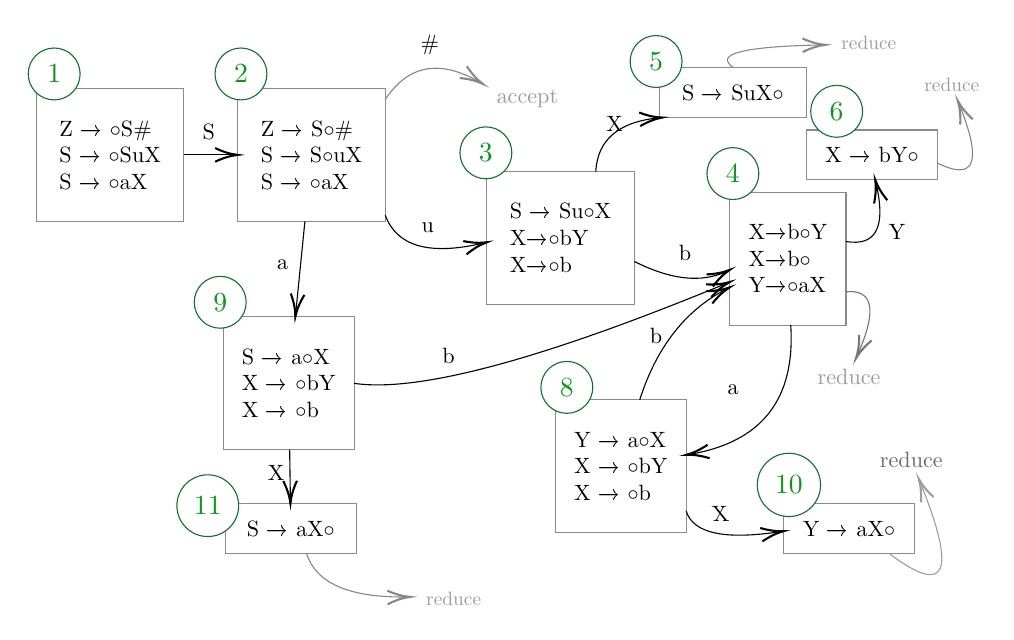
\begin{tikzpicture}[x=0.75pt,y=0.75pt,yscale=-1,xscale=1]
%uncomment if require: \path (0,283); %set diagram left start at 0, and has height of 283


% Text Node
\draw  [color={rgb, 255:red, 139; green, 139; blue, 139 }  ,draw opacity=1 ]  (8,28) -- (79,28) -- (79,92) -- (8,92) -- cycle  ;
\draw (43.5,60) node [scale=0.8,color={rgb, 255:red, 0; green, 0; blue, 0 }  ,opacity=1 ] [align=left] {Z → $\displaystyle \circ $S\#\\S → $\displaystyle \circ $SuX\\S → $\displaystyle \circ $aX};
% Text Node
\draw  [color={rgb, 255:red, 139; green, 139; blue, 139 }  ,draw opacity=1 ]  (105,28) -- (176,28) -- (176,92) -- (105,92) -- cycle  ;
\draw (140.5,60) node [scale=0.8,color={rgb, 255:red, 0; green, 0; blue, 0 }  ,opacity=1 ] [align=left] {Z → S$\displaystyle \circ $\#\\S → S$\displaystyle \circ $uX\\S → $\displaystyle \circ $aX};
% Text Node
\draw  [color={rgb, 255:red, 139; green, 139; blue, 139 }  ,draw opacity=1 ]  (225,68) -- (296,68) -- (296,132) -- (225,132) -- cycle  ;
\draw (260.5,100) node [scale=0.8,color={rgb, 255:red, 0; green, 0; blue, 0 }  ,opacity=1 ] [align=left] {S → Su$\displaystyle \circ $X\\X→$\displaystyle \circ $bY\\X→$\displaystyle \circ $b};
% Text Node
\draw  [color={rgb, 255:red, 139; green, 139; blue, 139 }  ,draw opacity=1 ]  (342,78) -- (398,78) -- (398,142) -- (342,142) -- cycle  ;
\draw (370,110) node [scale=0.8,color={rgb, 255:red, 0; green, 0; blue, 0 }  ,opacity=1 ] [align=left] {X→b$\displaystyle \circ $Y\\X→b$\displaystyle \circ $\\Y→$\displaystyle \circ $aX};
% Text Node
\draw (244.5,33) node [scale=0.8,color={rgb, 255:red, 156; green, 156; blue, 156 }  ,opacity=1 ] [align=left] {accept};
% Text Node
\draw (91,49) node [scale=0.8] [align=left] {S};
% Text Node
\draw (197.5,7) node [scale=0.8] [align=left] {\#};
% Text Node
\draw (320.5,107) node [scale=0.8] [align=left] {b};
% Text Node
\draw (343.5,173) node [scale=0.8] [align=left] {a};
% Text Node
\draw (399.5,167) node [scale=0.8,color={rgb, 255:red, 156; green, 156; blue, 156 }  ,opacity=1 ] [align=left] {reduce};
% Text Node
\draw (337.5,233) node [scale=0.8,xslant=-0.14] [align=left] {X};
% Text Node
\draw (196.5,95) node [scale=0.8] [align=left] {u};
% Text Node
\draw  [color={rgb, 255:red, 139; green, 139; blue, 139 }  ,draw opacity=1 ]  (308,18) -- (379,18) -- (379,42) -- (308,42) -- cycle  ;
\draw (343.5,30) node [scale=0.8,color={rgb, 255:red, 0; green, 0; blue, 0 }  ,opacity=1 ] [align=left] {S → SuX$\displaystyle \circ $};
% Text Node
\draw (286.5,45) node [scale=0.8] [align=left] {X};
% Text Node
\draw  [color={rgb, 255:red, 139; green, 139; blue, 139 }  ,draw opacity=1 ]  (258,178) -- (321,178) -- (321,242) -- (258,242) -- cycle  ;
\draw (289.5,210) node [scale=0.8,color={rgb, 255:red, 0; green, 0; blue, 0 }  ,opacity=1 ] [align=left] {Y → a$\displaystyle \circ $X\\X → $\displaystyle \circ $bY\\X → $\displaystyle \circ $b};
% Text Node
\draw (306.5,147) node [scale=0.8] [align=left] {b};
% Text Node
\draw  [color={rgb, 255:red, 139; green, 139; blue, 139 }  ,draw opacity=1 ]  (379,48) -- (442,48) -- (442,72) -- (379,72) -- cycle  ;
\draw (410.5,60) node [scale=0.8,color={rgb, 255:red, 0; green, 0; blue, 0 }  ,opacity=1 ] [align=left] {X → bY$\displaystyle \circ $};
% Text Node
\draw (422.5,97) node [scale=0.8] [align=left] {Y};
% Text Node
\draw (449,26) node [scale=0.7,color={rgb, 255:red, 156; green, 156; blue, 156 }  ,opacity=1 ] [align=left] {reduce};
% Text Node
\draw  [color={rgb, 255:red, 139; green, 139; blue, 139 }  ,draw opacity=1 ]  (98,138) -- (161,138) -- (161,202) -- (98,202) -- cycle  ;
\draw (129.5,170) node [scale=0.8,color={rgb, 255:red, 0; green, 0; blue, 0 }  ,opacity=1 ] [align=left] {S → a$\displaystyle \circ $X\\X → $\displaystyle \circ $bY\\X → $\displaystyle \circ $b};
% Text Node
\draw (206.5,157) node [scale=0.8] [align=left] {b};
% Text Node
\draw (126.5,113) node [scale=0.8] [align=left] {a};
% Text Node
\draw  [color={rgb, 255:red, 139; green, 139; blue, 139 }  ,draw opacity=1 ]  (99,228) -- (162,228) -- (162,252) -- (99,252) -- cycle  ;
\draw (130.5,240) node [scale=0.8,color={rgb, 255:red, 0; green, 0; blue, 0 }  ,opacity=1 ] [align=left] {S → aX$\displaystyle \circ $};
% Text Node
\draw (209,274) node [scale=0.7,color={rgb, 255:red, 156; green, 156; blue, 156 }  ,opacity=1 ] [align=left] {reduce};
% Text Node
\draw (123.5,213) node [scale=0.8] [align=left] {X};
% Text Node
\draw  [color={rgb, 255:red, 139; green, 139; blue, 139 }  ,draw opacity=1 ]  (368,228) -- (431,228) -- (431,252) -- (368,252) -- cycle  ;
\draw (399.5,240) node [scale=0.8,color={rgb, 255:red, 0; green, 0; blue, 0 }  ,opacity=1 ] [align=left] {Y → aX$\displaystyle \circ $};
% Text Node
\draw (429.5,207) node [scale=0.8,color={rgb, 255:red, 107; green, 107; blue, 107 }  ,opacity=1 ] [align=left] {reduce};
% Text Node
\draw (409,6) node [scale=0.7,color={rgb, 255:red, 156; green, 156; blue, 156 }  ,opacity=1 ] [align=left] {reduce};
% Text Node
\draw  [color={rgb, 255:red, 13; green, 116; blue, 41 }  ,draw opacity=1 ][fill={rgb, 255:red, 255; green, 255; blue, 255 }  ,fill opacity=1 ]  (16.5, 21) circle [x radius= 12.5, y radius= 12.5]   ;
\draw (16.5,21) node [color={rgb, 255:red, 11; green, 151; blue, 25 }  ,opacity=1 ] [align=left] {1};
% Text Node
\draw  [color={rgb, 255:red, 13; green, 116; blue, 41 }  ,draw opacity=1 ][fill={rgb, 255:red, 255; green, 255; blue, 255 }  ,fill opacity=1 ]  (106.5, 21) circle [x radius= 12.5, y radius= 12.5]   ;
\draw (106.5,21) node [color={rgb, 255:red, 11; green, 151; blue, 25 }  ,opacity=1 ] [align=left] {2};
% Text Node
\draw  [color={rgb, 255:red, 13; green, 116; blue, 41 }  ,draw opacity=1 ][fill={rgb, 255:red, 255; green, 255; blue, 255 }  ,fill opacity=1 ]  (224.5, 59) circle [x radius= 12.5, y radius= 12.5]   ;
\draw (224.5,59) node [color={rgb, 255:red, 11; green, 151; blue, 25 }  ,opacity=1 ] [align=left] {3};
% Text Node
\draw  [color={rgb, 255:red, 13; green, 116; blue, 41 }  ,draw opacity=1 ][fill={rgb, 255:red, 255; green, 255; blue, 255 }  ,fill opacity=1 ]  (343.5, 69) circle [x radius= 12.5, y radius= 12.5]   ;
\draw (343.5,69) node [color={rgb, 255:red, 11; green, 151; blue, 25 }  ,opacity=1 ] [align=left] {4};
% Text Node
\draw  [color={rgb, 255:red, 13; green, 116; blue, 41 }  ,draw opacity=1 ][fill={rgb, 255:red, 255; green, 255; blue, 255 }  ,fill opacity=1 ]  (306.5, 15) circle [x radius= 12.5, y radius= 12.5]   ;
\draw (306.5,15) node [color={rgb, 255:red, 11; green, 151; blue, 25 }  ,opacity=1 ] [align=left] {5};
% Text Node
\draw  [color={rgb, 255:red, 13; green, 116; blue, 41 }  ,draw opacity=1 ][fill={rgb, 255:red, 255; green, 255; blue, 255 }  ,fill opacity=1 ]  (393.5, 39) circle [x radius= 12.5, y radius= 12.5]   ;
\draw (393.5,39) node [color={rgb, 255:red, 11; green, 151; blue, 25 }  ,opacity=1 ] [align=left] {6};
% Text Node
\draw  [color={rgb, 255:red, 13; green, 116; blue, 41 }  ,draw opacity=1 ][fill={rgb, 255:red, 255; green, 255; blue, 255 }  ,fill opacity=1 ]  (263.5, 172) circle [x radius= 12.5, y radius= 12.5]   ;
\draw (263.5,172) node [color={rgb, 255:red, 11; green, 151; blue, 25 }  ,opacity=1 ] [align=left] {8};
% Text Node
\draw  [color={rgb, 255:red, 13; green, 116; blue, 41 }  ,draw opacity=1 ][fill={rgb, 255:red, 255; green, 255; blue, 255 }  ,fill opacity=1 ]  (96.5, 131) circle [x radius= 12.5, y radius= 12.5]   ;
\draw (96.5,131) node [color={rgb, 255:red, 11; green, 151; blue, 25 }  ,opacity=1 ] [align=left] {9};
% Text Node
\draw  [color={rgb, 255:red, 13; green, 116; blue, 41 }  ,draw opacity=1 ][fill={rgb, 255:red, 255; green, 255; blue, 255 }  ,fill opacity=1 ]  (370.5, 219) circle [x radius= 15.24, y radius= 15.24]   ;
\draw (370.5,219) node [color={rgb, 255:red, 11; green, 151; blue, 25 }  ,opacity=1 ] [align=left] {10};
% Text Node
\draw  [color={rgb, 255:red, 13; green, 116; blue, 41 }  ,draw opacity=1 ][fill={rgb, 255:red, 255; green, 255; blue, 255 }  ,fill opacity=1 ]  (90.5, 229) circle [x radius= 14.87, y radius= 14.87]   ;
\draw (90.5,229) node [color={rgb, 255:red, 11; green, 151; blue, 25 }  ,opacity=1 ] [align=left] {11};
% Connection
\draw    (79,60) -- (103,60) ;
\draw [shift={(105,60)}, rotate = 180] [color={rgb, 255:red, 0; green, 0; blue, 0 }  ][line width=0.75]    (10.93,-3.29) .. controls (6.95,-1.4) and (3.31,-0.3) .. (0,0) .. controls (3.31,0.3) and (6.95,1.4) .. (10.93,3.29)   ;

% Connection
\draw    (176,89.04) .. controls (181.56,104.13) and (197.36,108.61) .. (223.39,102.47) ;
\draw [shift={(225,102.08)}, rotate = 526.04] [color={rgb, 255:red, 0; green, 0; blue, 0 }  ][line width=0.75]    (10.93,-3.29) .. controls (6.95,-1.4) and (3.31,-0.3) .. (0,0) .. controls (3.31,0.3) and (6.95,1.4) .. (10.93,3.29)   ;

% Connection
\draw    (296,111.32) .. controls (313.43,120.16) and (328.19,121.8) .. (340.31,116.23) ;
\draw [shift={(342,115.39)}, rotate = 512.21] [color={rgb, 255:red, 0; green, 0; blue, 0 }  ][line width=0.75]    (10.93,-3.29) .. controls (6.95,-1.4) and (3.31,-0.3) .. (0,0) .. controls (3.31,0.3) and (6.95,1.4) .. (10.93,3.29)   ;

% Connection
\draw [color={rgb, 255:red, 134; green, 134; blue, 134 }  ,draw opacity=1 ]   (176,33.36) .. controls (186.96,16.6) and (202.13,13.79) .. (221.5,24.91) ;
\draw [shift={(223,25.79)}, rotate = 211.15] [color={rgb, 255:red, 134; green, 134; blue, 134 }  ,draw opacity=1 ][line width=0.75]    (10.93,-3.29) .. controls (6.95,-1.4) and (3.31,-0.3) .. (0,0) .. controls (3.31,0.3) and (6.95,1.4) .. (10.93,3.29)   ;

% Connection
\draw [color={rgb, 255:red, 117; green, 117; blue, 117 }  ,draw opacity=1 ]   (398,125.95) .. controls (411.22,124.71) and (413.07,134.83) .. (403.56,156.32) ;
\draw [shift={(402.8,158)}, rotate = 294.58] [color={rgb, 255:red, 117; green, 117; blue, 117 }  ,draw opacity=1 ][line width=0.75]    (10.93,-3.29) .. controls (6.95,-1.4) and (3.31,-0.3) .. (0,0) .. controls (3.31,0.3) and (6.95,1.4) .. (10.93,3.29)   ;

% Connection
\draw    (277.44,68) .. controls (278.29,52.74) and (288.38,44.13) .. (307.69,42.16) ;
\draw [shift={(309.5,42)}, rotate = 535.54] [color={rgb, 255:red, 0; green, 0; blue, 0 }  ][line width=0.75]    (10.93,-3.29) .. controls (6.95,-1.4) and (3.31,-0.3) .. (0,0) .. controls (3.31,0.3) and (6.95,1.4) .. (10.93,3.29)   ;

% Connection
\draw    (371.37,142) .. controls (373.69,177.69) and (357.44,198.45) .. (322.6,204.28) ;
\draw [shift={(321,204.53)}, rotate = 351.37] [color={rgb, 255:red, 0; green, 0; blue, 0 }  ][line width=0.75]    (10.93,-3.29) .. controls (6.95,-1.4) and (3.31,-0.3) .. (0,0) .. controls (3.31,0.3) and (6.95,1.4) .. (10.93,3.29)   ;

% Connection
\draw    (298.62,178) .. controls (306.74,152.56) and (320.69,134.76) .. (340.47,124.57) ;
\draw [shift={(342,123.8)}, rotate = 513.98] [color={rgb, 255:red, 0; green, 0; blue, 0 }  ][line width=0.75]    (10.93,-3.29) .. controls (6.95,-1.4) and (3.31,-0.3) .. (0,0) .. controls (3.31,0.3) and (6.95,1.4) .. (10.93,3.29)   ;

% Connection
\draw    (398,101.72) .. controls (412.54,104.14) and (417.36,94.78) .. (412.48,73.65) ;
\draw [shift={(412.08,72)}, rotate = 436.1] [color={rgb, 255:red, 0; green, 0; blue, 0 }  ][line width=0.75]    (10.93,-3.29) .. controls (6.95,-1.4) and (3.31,-0.3) .. (0,0) .. controls (3.31,0.3) and (6.95,1.4) .. (10.93,3.29)   ;

% Connection
\draw [color={rgb, 255:red, 134; green, 134; blue, 134 }  ,draw opacity=1 ]   (442,63.91) .. controls (460.24,72.88) and (463.76,63.48) .. (452.59,35.72) ;
\draw [shift={(451.89,34)}, rotate = 427.56] [color={rgb, 255:red, 134; green, 134; blue, 134 }  ,draw opacity=1 ][line width=0.75]    (10.93,-3.29) .. controls (6.95,-1.4) and (3.31,-0.3) .. (0,0) .. controls (3.31,0.3) and (6.95,1.4) .. (10.93,3.29)   ;

% Connection
\draw    (137.3,92) -- (132.9,136.01) ;
\draw [shift={(132.7,138)}, rotate = 275.71] [color={rgb, 255:red, 0; green, 0; blue, 0 }  ][line width=0.75]    (10.93,-3.29) .. controls (6.95,-1.4) and (3.31,-0.3) .. (0,0) .. controls (3.31,0.3) and (6.95,1.4) .. (10.93,3.29)   ;

% Connection
\draw    (161,170.06) .. controls (191.85,174.63) and (251.75,158.53) .. (340.66,121.79) ;
\draw [shift={(342,121.23)}, rotate = 517.5] [color={rgb, 255:red, 0; green, 0; blue, 0 }  ][line width=0.75]    (10.93,-3.29) .. controls (6.95,-1.4) and (3.31,-0.3) .. (0,0) .. controls (3.31,0.3) and (6.95,1.4) .. (10.93,3.29)   ;

% Connection
\draw    (129.96,202) -- (130.3,226) ;
\draw [shift={(130.33,228)}, rotate = 269.18] [color={rgb, 255:red, 0; green, 0; blue, 0 }  ][line width=0.75]    (10.93,-3.29) .. controls (6.95,-1.4) and (3.31,-0.3) .. (0,0) .. controls (3.31,0.3) and (6.95,1.4) .. (10.93,3.29)   ;

% Connection
\draw [color={rgb, 255:red, 134; green, 134; blue, 134 }  ,draw opacity=1 ]   (138.07,252) .. controls (142.6,266.38) and (158.67,273.37) .. (186.29,272.98) ;
\draw [shift={(188,272.95)}, rotate = 538.5899999999999] [color={rgb, 255:red, 134; green, 134; blue, 134 }  ,draw opacity=1 ][line width=0.75]    (10.93,-3.29) .. controls (6.95,-1.4) and (3.31,-0.3) .. (0,0) .. controls (3.31,0.3) and (6.95,1.4) .. (10.93,3.29)   ;

% Connection
\draw    (321,231.58) .. controls (324.26,242.31) and (339.38,245.62) .. (366.33,241.52) ;
\draw [shift={(368,241.26)}, rotate = 530.89] [color={rgb, 255:red, 0; green, 0; blue, 0 }  ][line width=0.75]    (10.93,-3.29) .. controls (6.95,-1.4) and (3.31,-0.3) .. (0,0) .. controls (3.31,0.3) and (6.95,1.4) .. (10.93,3.29)   ;

% Connection
\draw [color={rgb, 255:red, 158; green, 158; blue, 158 }  ,draw opacity=1 ]   (418.79,252) .. controls (446.65,273.12) and (451.57,261.57) .. (433.57,217.35) ;
\draw [shift={(433.02,216)}, rotate = 427.63] [color={rgb, 255:red, 158; green, 158; blue, 158 }  ,draw opacity=1 ][line width=0.75]    (10.93,-3.29) .. controls (6.95,-1.4) and (3.31,-0.3) .. (0,0) .. controls (3.31,0.3) and (6.95,1.4) .. (10.93,3.29)   ;

% Connection
\draw [color={rgb, 255:red, 136; green, 136; blue, 136 }  ,draw opacity=1 ]   (343.86,18) .. controls (334.1,11.43) and (348.23,7.77) .. (386.25,7.02) ;
\draw [shift={(388,6.98)}, rotate = 539.01] [color={rgb, 255:red, 136; green, 136; blue, 136 }  ,draw opacity=1 ][line width=0.75]    (10.93,-3.29) .. controls (6.95,-1.4) and (3.31,-0.3) .. (0,0) .. controls (3.31,0.3) and (6.95,1.4) .. (10.93,3.29)   ;


\end{tikzpicture}


\end{figure}

Nie ma konfliktów, więc jest SLR(1)

\subsubsection{LALR(1) / LR(1)}

[uwaga - zmieniamy gramatykę - tamta jest już SLR(1), więc nie ma sensu rozpatrywać czy jest LALR(1)]

Zamiast patrzeć przy redukcjach na globalne zbiory follow, patrzymy na "lokalny" przyszłości, tzn. dopełniając regułę $X \ra \alpha \circ B \beta, \{a \}$, zbiór przyszłości rozwiniętej reguły $B$ to $First(\beta)$, a jeśli $\beta$ jest nullowalne, to także przyszłość reguły $X$.

Po konstrukcji automaty LR(1) możemy skleić te same stany (przy sklejaniu nie patrzymy na przyszłość: po prostu jeśli dwa stany mają dokładnie te same stany, z dokładnością do kropek, można skleić) tworząc automat LALR(1). Nie zawsze jest to możliwe, tzn. po sklejeniu tych ,,samych stanów'' mogą pojawić się konflikty, wtedy gramatyka jest LR(1), ale nie LALR(1).

\tikzset{every picture/.style={line width=0.75pt}} %set default line width to 0.75pt        

\begin{tikzpicture}[x=0.75pt,y=0.75pt,yscale=-1,xscale=1]
%uncomment if require: \path (0,412); %set diagram left start at 0, and has height of 412

%Straight Lines [id:da7411648470074887] 
\draw [color={rgb, 255:red, 0; green, 158; blue, 255 }  ,draw opacity=1 ]   (392,218) -- (243.55,96.27) ;
\draw [shift={(242,95)}, rotate = 399.35] [color={rgb, 255:red, 0; green, 158; blue, 255 }  ,draw opacity=1 ][line width=0.75]    (10.93,-3.29) .. controls (6.95,-1.4) and (3.31,-0.3) .. (0,0) .. controls (3.31,0.3) and (6.95,1.4) .. (10.93,3.29)   ;

%Straight Lines [id:da740624439381262] 
\draw [color={rgb, 255:red, 0; green, 158; blue, 255 }  ,draw opacity=1 ]   (392,218) -- (265.89,173.66) ;
\draw [shift={(264,173)}, rotate = 379.37] [color={rgb, 255:red, 0; green, 158; blue, 255 }  ,draw opacity=1 ][line width=0.75]    (10.93,-3.29) .. controls (6.95,-1.4) and (3.31,-0.3) .. (0,0) .. controls (3.31,0.3) and (6.95,1.4) .. (10.93,3.29)   ;


% Text Node
\draw    (23.5,126) -- (112.5,126) -- (112.5,256) -- (23.5,256) -- cycle  ;
\draw (68,191) node  [align=left] {Z → .S\#, \_\\S → .Aa, \#\\S → .bAc, \#\\S → .Bc, \#\\S → .bBa, \#\\A → .d, a\\B → .d, c};
% Text Node
\draw    (172,53) -- (242,53) -- (242,93) -- (172,93) -- cycle  ;
\draw (207,73) node  [align=left] {A → d., a\\B → d., c};
% Text Node
\draw (296,27) node  [align=left] {to nie SLR(1), bo tu\\mamy konflikt Reduce-Reduce};
% Text Node
\draw (371,65) node  [align=left] {reduce(A → d)};
% Text Node
\draw (372,87) node  [align=left] {reduce(B → d)};
% Text Node
\draw (300,64) node  [align=left] {a\\c};
% Text Node
\draw (138,111) node  [align=left] {d};
% Text Node
\draw    (184.5,220) -- (273.5,220) -- (273.5,296) -- (184.5,296) -- cycle  ;
\draw (229,258) node  [align=left] {S → b.Ac, \#\\S → b.Ba, \#\\A → .d, c\\B → .d, a};
% Text Node
% wersja sprzed czasów Andrzeja
% \draw    (157.5,322) -- (246.5,322) -- (246.5,362) -- (157.5,362) -- cycle  ;
% \draw (202,342) node  [align=left] {S → a.Aa, \#\\A → .d, a};
% Text Node
\draw    (101,381) -- (181,381) -- (181,403) -- (101,403) -- cycle  ;
\draw (141,392) node  [align=left] {Z → S.\#, \_};
% Text Node
\draw    (192.5,135) -- (263.5,135) -- (263.5,175) -- (192.5,175) -- cycle  ;
\draw (228,155) node  [align=left] {A → d., c\\B → d., a};
% Text Node
\draw (365,147) node  [align=left] {reduce(A → d)};
% Text Node
\draw (366,169) node  [align=left] {reduce(B → d)};
% Text Node
\draw (296,151) node  [align=left] {c\\a};
% Text Node
\draw (410,263) node  [align=left] {Gdybyśmy skleili te stany (bo\\mają te same, reguły (razem\\z kropkami!)) to byłby konflikt\\po literce a byłyby dwie redukcje\\(to samo po literce c)\\dlatego to nie LALR(1)};
% Connection
\draw    (242,71.29) -- (316.5,67.66) ;
\draw [shift={(318.5,67.56)}, rotate = 537.21] [color={rgb, 255:red, 0; green, 0; blue, 0 }  ][line width=0.75]    (10.93,-3.29) .. controls (6.95,-1.4) and (3.31,-0.3) .. (0,0) .. controls (3.31,0.3) and (6.95,1.4) .. (10.93,3.29)   ;

% Connection
\draw    (242,75.97) -- (317.01,82.33) ;
\draw [shift={(319,82.5)}, rotate = 184.85] [color={rgb, 255:red, 0; green, 0; blue, 0 }  ][line width=0.75]    (10.93,-3.29) .. controls (6.95,-1.4) and (3.31,-0.3) .. (0,0) .. controls (3.31,0.3) and (6.95,1.4) .. (10.93,3.29)   ;

% Connection
\draw    (112.5,153.22) -- (181.92,94.29) ;
\draw [shift={(183.44,93)}, rotate = 499.67] [color={rgb, 255:red, 0; green, 0; blue, 0 }  ][line width=0.75]    (10.93,-3.29) .. controls (6.95,-1.4) and (3.31,-0.3) .. (0,0) .. controls (3.31,0.3) and (6.95,1.4) .. (10.93,3.29)   ;

% Connection
\draw    (112.5,209.52) -- (182.65,238.71) ;
\draw [shift={(184.5,239.48)}, rotate = 202.59] [color={rgb, 255:red, 0; green, 0; blue, 0 }  ][line width=0.75]    (10.93,-3.29) .. controls (6.95,-1.4) and (3.31,-0.3) .. (0,0) .. controls (3.31,0.3) and (6.95,1.4) .. (10.93,3.29)   ;

% Connection
\draw    (228.63,220) -- (228.21,177) ;
\draw [shift={(228.19,175)}, rotate = 449.44] [color={rgb, 255:red, 0; green, 0; blue, 0 }  ][line width=0.75]    (10.93,-3.29) .. controls (6.95,-1.4) and (3.31,-0.3) .. (0,0) .. controls (3.31,0.3) and (6.95,1.4) .. (10.93,3.29)   ;

% Connection
\draw    (263.5,158.6) -- (311.01,163.42) ;
\draw [shift={(313,163.62)}, rotate = 185.79] [color={rgb, 255:red, 0; green, 0; blue, 0 }  ][line width=0.75]    (10.93,-3.29) .. controls (6.95,-1.4) and (3.31,-0.3) .. (0,0) .. controls (3.31,0.3) and (6.95,1.4) .. (10.93,3.29)   ;

% Connection
\draw    (263.5,152.93) -- (310.5,150.18) ;
\draw [shift={(312.5,150.07)}, rotate = 536.6600000000001] [color={rgb, 255:red, 0; green, 0; blue, 0 }  ][line width=0.75]    (10.93,-3.29) .. controls (6.95,-1.4) and (3.31,-0.3) .. (0,0) .. controls (3.31,0.3) and (6.95,1.4) .. (10.93,3.29)   ;

% wersja sprzed czasów Andrzeja
% Connection
% \draw    (112.5,241.15) -- (182.92,320.5) ;
% \draw [shift={(184.25,322)}, rotate = 228.41] [color={rgb, 255:red, 0; green, 0; blue, 0 }  ][line width=0.75]    (10.93,-3.29) .. controls (6.95,-1.4) and (3.31,-0.3) .. (0,0) .. controls (3.31,0.3) and (6.95,1.4) .. (10.93,3.29)   ;

% Connection
\draw    (91.61,256) -- (136.32,379.12) ;
\draw [shift={(137,381)}, rotate = 250.04000000000002] [color={rgb, 255:red, 0; green, 0; blue, 0 }  ][line width=0.75]    (10.93,-3.29) .. controls (6.95,-1.4) and (3.31,-0.3) .. (0,0) .. controls (3.31,0.3) and (6.95,1.4) .. (10.93,3.29)   ;


\end{tikzpicture}

\subsubsection{Co z $\varepsilon$ w produkcji?}

Nic, po prostu nic nie piszemy i z produkcji $A \rightarrow \varepsilon$, w grafie pojawi się $A \rightarrow \circ $, po której od razu robimy redukcję (nie ma przejść po $\varepsilon$, od razu redukcja).

\section{Gramatyki atrybutywne}

    Do symboli (nieterminali i terminali) w gramatyce dodajemy \textsc{atrybuty}, tj. informację, jaką ze sobą ten symbol niesie.

\begin{itemize}
    \item atrybuty syntezowane
    
    gdy mamy produkcję $X \ra \alpha$ i ustawiamy atrybut nieterminalowi po lewej stronie - X. Ten atrybut będzie propagowany w górę. 
    
    \item atrybuty dziedziczone
    
    gdy mamy produkcję $X \ra \alpha Y \beta$ i ustawiamy atrybut nieterminalowi po prawej stronie - Y. Ten atrybut będzie propagowany w dół (gdy będziemy parsować $Y \ra \gamma$, ten nieterminal może się dowiedzieć co przyszło do niego z góry)
    
    \item atrybuty wbudowane - atrybuty nadawane terminalom (identyczne zasady)
\end{itemize}

\textsc{Przykład}:

$\quad Z \ra S$

$\quad S \ra X | XS$

$\quad X \ra ab | aXb$

Chcemy nadać atrybut $Z.ak$ na true wtw gdy słowo $w$ jest postaci $(a^nb^n)^n$

$\quad Z \ra S$   \{$Z.ok = S.ileX == S.\#ab\ and\ S.ok$\}

$\quad S \ra X$    \{$S.ileX = 1$, $S.\#ab = X_0.ile$, $S.ok = true$\}

$\quad S_0 \ra XS_1$ \{$S_0.ileX = 1 + S_1.ileX$, $S_0.ok = S_1.ok\ and\ X.ile == S1.\#ab$, $S_0.\#ab = S_1.\#ab$\}

$\quad X \ra ab$ \{$X.ile = 1$\}

$\quad X_0 \ra aX_1b$ \{$X_0.ile = 1 + X_1.ile$\}

$X.ile$ - ile wynosi $k$ w wyprodukowanym $a^kb^k$

$S.ileX$ - ile Xów wyprodukowało S

$S.ok$ - czy wszystkie X które ten S wyprowadził, $X.ile$ ma tę samą wartość

$S.\#ab$ - jaką wartość ma $X.ile$, którą wyprowadził (bo każdy X ma mieć tę samą)


\section{SSA oraz optymalizacje}

    
\subsection{Ogólnie optymalizacje}

\begin{itemize}
    \item \textsc{Constant folding/propagation}

\begin{figure}[H]
 \begin{minipage}{0.1\textwidth}
  \centering
  \begin{minted}{python}
t1 := 7
t2 := t1 - 1
t3 := t2 * t2
a := b + t3
  \end{minted}
 \end{minipage}
 \begin{minipage}{0.04\textwidth}
 $\rightarrow$
 \end{minipage}
 \begin{minipage}{0.2\textwidth}
  \centering
  \begin{minted}{python}
a := b + 36
  \end{minted}
 \end{minipage}
\end{figure}

\begin{figure}[H]
 \begin{minipage}{0.2\textwidth}
  \centering
  \begin{minted}{python}
r1 := 1
...
r5 = phi(entry: r1, L5: r7) 
  \end{minted}
 \end{minipage}
 \begin{minipage}{0.04\textwidth}
 $\rightarrow$
 \end{minipage}
 \begin{minipage}{0.2\textwidth}
  \centering
  \begin{minted}{python}
r1 := 1
...
r5 = phi(entry: 1, L5: r7) 
  \end{minted}
 \end{minipage}
\end{figure}

\item \textsc{Copy propagation}

\begin{figure}[H]
 \begin{minipage}{0.1\textwidth}
  \centering
  \begin{minted}{python}
x := y
t := x + 1
  \end{minted}
 \end{minipage}
 \begin{minipage}{0.04\textwidth}
 $\rightarrow$
 \end{minipage}
 \begin{minipage}{0.2\textwidth}
  \centering
  \begin{minted}{python}
x := y
t := y + 1
  \end{minted}
 \end{minipage}
\end{figure}

\item \textsc{Local Common Subexpression Elimination}

\begin{figure}[H]
 \begin{minipage}{0.1\textwidth}
  \centering
  \begin{minted}{python}
t6 := 4*i
x := a[t6]
t7 := 4*i
t8 := 4*j
t9 := a[t8]
a[t7] := t9
t10 := 4*j
a[t10] := x
goto L5
  \end{minted}
 \end{minipage}
 \begin{minipage}{0.04\textwidth}
 $\rightarrow$
 \end{minipage}
 \begin{minipage}{0.2\textwidth}
  \centering
  \begin{minted}{python}
t6 := 4*i
x := a[t6]

t8 := 4*j
t9 := a[t8]
a[t6] := t9

a[t8] := x
goto L5
  \end{minted}
 \end{minipage}
\end{figure}

\item \textsc{Global Common Subexpression Elimination}

To samo, ale między blokami prostymi

\item \textsc{Dead Code Elimination}

Wywalamy nieużywane rejestry

\item \textsc{Moving code out of the loop}

\begin{figure}[H]
 \begin{minipage}{0.15\textwidth}
  \centering
  \begin{minted}{c}
  |$\ $|
while(i<=n-3) {
    s += a[i];
    i++;
}

  \end{minted}
 \end{minipage}
 \begin{minipage}{0.04\textwidth}
 $\rightarrow$
 \end{minipage}
 \begin{minipage}{0.2\textwidth}
  \centering
  \begin{minted}{python}
t = n-3;
while(i<=t) {
    s += a[i];
    i++;
}
  \end{minted}
 \end{minipage}
\end{figure}

\item \textsc{Strength reduction} - zastępowanie drogich operacji prostszymi (np. mnożenie dodawaniem)

\begin{figure}[H]
 \begin{minipage}{0.15\textwidth}
  \centering
  \begin{minted}{c}
    i := 0;
goto L2
L1: i := i+1
    t2 := 4*i
    t3 := a[t2]
    s := s + t3
L2: if(a[t2]<=k) goto L1

  \end{minted}
 \end{minipage}
 \begin{minipage}{0.04\textwidth}
 $\rightarrow$
 \end{minipage}
 \begin{minipage}{0.2\textwidth}
  \centering
  \begin{minted}{python}
    t2 := 0;
    goto L2
L1: t2 := t2 + 4 
    t3 := a[t2]
    s := s + t3
L2: if(a[t2]<=k) goto L1

  \end{minted}
 \end{minipage}
\end{figure}

\item \textsc{Loop unrolling, loop inlining}

Loop unrolling - zmniejszenie liczby obrotów poprzez wykonywanie kilku obrotów pętli na raz (np. na x86 zamiast robić strcmp na bajtach - robić na całych słowach)

Loop inlining - unrolling do zera

\end{itemize}

\subsection{Przykład:}


\begin{minted}{c}
for (m = a[i]; (i > 0) && (3 + m < a[i-]); i--)
    a[i] = a[i-1];
a[i] = m;
        czwórkowy:                      SSA
 1. L0:                             L0:
 2.    m = a[i]                       m = a[i]
 3. L1:                             L1:
 4.     if i > 0 goto L2 else L3       i1 = |$\phi$|(L0: i, L4: i2)
 5.                                    if i1 > 0 goto L2 else L3
 6. l2:                             L2:
 7.     t1 = 3 + m                     t1 = 3 + m
 8.     t2 = i - 1                     t2 = i1 - 1
 9.     t3 = a[t2]                     t3 = a[t2]
10.     if t1 < t3 goto L4 else L3     if t1 < t3 goto L4 else L3
11. L4:                             L4:
12.     t4 = i - 1                     t4 = i1 - 1
13.     t5 = a[t4]                     t5 = a[t4]
14.     a[i] = t5                      a[i1] = t5
15.     i = i - 1                      i2 = i1 - 1
16.     goto L1                        goto L1
17. L3:                             L3:
18.      a[i] = m                      a[i1] = m
\end{minted}

\begin{enumerate}
    \item const folding: stałe wyliczamy w czasie kompilacji
    \item common subexpression substitution: tam gdzie występuje to samo, redukujemy (ale tylko obliczenia), np. w linijce 12 i 15 wyliczamy $i1 - 1$, które zostało już policzone w linijce 8. Uwaga na tablice!
    
    \item copy propagation:
    
    widzimy $y$ po prawej stronie równości
    
    szukamy $y = a$ (gdzie a jest po prostu rejestrem)
    
    zamieniamy $y$ na $a$
    
    \begin{minted}{c}
                     krok 2   krok 3       krok 2     krok 3
 1. L0:
 2.   m = a[i]
 3. L1:
 4.    i1 = |$\phi$|(L0: i, L4: i2)
 5.    if i1 > 0 
        goto L2 else L3
 6. L2:
 7.    t1 = 3 + m
 8.    t2 = i1 - 1
 9.    t3 = a[t2]
10.    if t1 < t3
        goto L4 else L3
11. L4:
12.    t4 = i1 - 1    t4 = t2
13.    t5 = a[t4]              t5 = a[t2]   t5 = t3
14.    a[i1] = t5                                     a[i1] = t3
15.    i2 = i1 - 1    i2 = t2
16.    goto L1
17. L3:
18.    a[i1] = m    
    \end{minted}
    
    
    Teraz znowu powtarzamy te kroki aż nic się nie będzie zmieniało

    \item Dead code optimization i wywalamy 12, 13 linijkę
    \item Wyciąganie stałych wyrażeń przed pętlę
        \begin{minted}{c}
 1. L0:
 2.   m = a[i]
 3.   t1 = 3 + m     <- tutaj
 4. L1:
 5.    i1 = |$\phi$|(L0: i, L4: i2)   // <- phi(L0: i, L4: t2)
 6.    if i1 > 0 goto L2 else L3
 7. L2:
 8.    t2 = i1 - 1
 9.    t3 = a[t2]
10.    if t1 < t3 goto L4 else L3
11. L4:
12.    a[i1] = t3
13.    i2 = t2               // <- usuwamy
14.    goto L1
15. L3:
16.    a[i1] = m    
    \end{minted}
    
    Teraz możemy znowu rozpropagowac kopię i w linijce 5. użyć $t2$ zamiast $i2$ (a następnie w ramach usuwania martwego kodu usunąć przypisanie do $i2$)
    
    
\end{enumerate}


\section{Kod czwórkowy i rejestry}

    \subsection{Liczenie zbioru zmiennych żywych}
Jeśli za operacją $R_x = operacja(R_1, R_2)$ zbiór zmiennych żywych to $\mathcal{X}$, to przed tą operacją zbiór zmiennych żywych $\mathcal{Y} = \mathcal{X} - \{R_x\} \cup \{R_1, R_2\}$. \textbf{Uwaga!} W wyniku przypisań w tych zadaniach może się okazać, że liczymy kilka razy to samo (choć zmienne mają inne nazwy). Jeśli znajdziesz w tym zadaniu na egzaminie miejsce na optymalizację pewnie warto się zapytać czy należy to zrobić.

\begin{table}[H]
\begin{tabular}{p{0.06\textwidth}|p{0.07\textwidth}|p{0.04\textwidth}|p{0.04\textwidth}|p{0.04\textwidth}|p{0.04\textwidth}|p{0.04\textwidth}|p{0.04\textwidth}}
& & \multicolumn{2}{c}{Co jest w} & \multicolumn{4}{c}{Gdzie jest dana} \\
& & \multicolumn{2}{c}{danym rejestrze} & \multicolumn{4}{c}{zmienna} \\
\hline 
 quad & ASM & R0 & R1 & a & b & c & d \\
\hline 
  &  &  &  &  & B &  & D \\
\hline 
 a = b &  &  &  & B &  &  & D \\
\hline 
 b = d &  &  &  & B & D &  &  \\
\hline 
 d = a &  &  &  & B & D &  & B \\
\hline 
 d = b - d & R0 = D & b &  & B & D, R0 &  & B \\
\hline 
  & R1 = B & b & d, a & B, R1 & R0, D &  & R1, B \\
\hline 
  & R0 = R0-R1 & d & a & B, R1 & D &  & R0 \\
\hline 
 c = a - d   & R1 = R1 - R0 & d & c & & D & R1 & R0 \\
\hline 
  & C = R1 & d & c &  & D & R1, C  & R0 \\
\hline 
  & R1 = D & d & b &  & D, R1 & C  & R0 \\
\hline 
  & B = R1 & d & b &  & B, D, R1 & C & R0 \\
\hline 
  & D = R0 & d & b &  & B, R1 & C & R0, D 
\end{tabular}
\end{table}

\section{ASM i JVM}

    \subsection{x86}
\begin{minted}{c}
mov EAX, EBX             EAX = EBX
lea EAX, [4 * EBX]       EAX = 4 * EBX
add EAX, [EBP - 8]       EAX = EAX + wartość pod (EBP - 8)
cmp EAX, EBX             
jg label                 skok gdy EAX > EBX
jl label                 skok gdy EAX < EBX
jge label                skok gdy EAX >= EBX
jle label                skok gdy EAX <= EBX
je/jne label             
push ebp                 standardowy prolog
mov rbp, esp             standardowy prolog
leave                    standardowy epilog
ret                      standardowy epilog
imul EBX                 EDX:EAX = EAX * EBX
imul EBX, ECX            EDX:EAX = EBX * ECX
idiv ECX                 EAX = EDX:EAX / ECX, EDX = EDX:EAX % ECX
mul                      mnożenie bez znaku
div                      dzielenie bez znaku
not EAX                  EAX = ~EAX
neg EAX                  EAX = -EAX
\end{minted}

\subsubsection{Protokół wywołania GCC+libc (aka “cdecl”)}

\begin{itemize}
    \item rejestry: $EAX$, $ECX$, $EDX$, $EBX$, $ESP$, $EBP$, $ESI$, $EDI$
    \item $EAX$, $ECX$, $EDX$ - caller saved (== można je zmieniać w funkcji bez obaw)
    \item pozostałe - callee saved (nie można zmieniać bez przywrócenia starej wartości przed wyjściem)
    \item argumenty od końca (najpierw wkładamy ostatnie)
    \item wynik w $EAX$
    \item gcc wyrównuje stos do 16 bajtów, tzn. przed zrobieniem $call$ stos jest wyrównany, tzn. po $call$, $ESP \equiv 4  mod 16$, tzn. po $push\ ebp$: $ESP \equiv 8 mod 16$.
    \item ale slajdy mówią o wyrównaniu tylko w przypadku x86\_64
\end{itemize}

\subsubsection{x86\_64}
\begin{itemize}
    \item rejestry: $RAX$, $RBX$, $RCX$, $RDX$, $RBP$, $RSP$, $RSI$, $RDI$, $R8$, $R9$, $R10$, $R11$, $R12$, $R13$, $R14$, $R15$
    \item inty przekazywane w: $EDI$, $ESI$, $EDX$, $ECX$, $R8D$, $R9D$
    \item $RBP$, $RBX$ and $R12$ - $R15$ callee saved
    \item stos na pewno wyrównany
\end{itemize}


\subsection{JVM}
\begin{minted}{c}
iconst_0            push 0
istore_2            pop from stack to 2. local var
iload_3             push 3. local variable
if_icmpge           skacze gdy wartość głębsza jest >= wartości na topie
aload_0             załaduj tablicę ze zmiennej lokalnej 0
iaload              wczytaj wartość z tablicy (głębiej tablica)
iinc X Y            zwiększ zmienną lokalną X o Y
dup                 duplikuj ostatnią rzecz na stosie
dup2                duplikuje dwie rzeczy ze stosu
ifeq label          skacze gdy wartość na stosie == 0
iastore             zapisuje do tablicy (od góry: wartość, indeks, tablica)
bipush 123          umieszcza bajt na stosie
idiv, iadd, isub, imul
\end{minted}

    
korczyn; nie biorę odpowiedzialności za błęęędy

\end{document}
